\chapter{Diseño}  \label{disenyo}

Este capítulo abarca aquellos aspectos considerados durante la fase del diseño de la aplicación, desde sus versiones primitivas (diseño conceptual) hasta el diseño final de la aplicación, pasándo por los diferentes diagramas arquitecturales que muestran el sistema desde diferentes puntos de vista. Además, al final se hará una retrospectiva sobre aquellas restricciones que han afectado el curso del desarrollo de las diferentes soluciones desde el punto de vista del diseño. 


\section{Diseño conceptual} \label{disenyo.conceptual}
Con el análisis finalizado y teniéndo en cuenta los requisitos, se llegó a la conclusión de que los desarrollos realizados a lo largo de la duración de este proyecto no serían más que el comienzo para algo mucho más grande; se debía ofrecer tanto la infraestructura necesaria como el soporte para que la solución pudiera escalar y ser expandida mediante el trabajo de futuros desarrolladores. 


\par 
El diseño conceptual del sistema se presenta a continuación a una escala abstracta y de alto nivel. Básicamente, el proyecto hará uso de numerosas fuentes de información, en este caso sobre productos fitosanitarios y sus derivados. Dicha información deberá ser recogida de manera periódica y almacenada en algún sistema de persistencia tal como proviene de sus fuentes, es decir, en una versión \textit{en crudo}. Una vez almacenada en su versión original, los datos pasarán a una siguiente fase en la que serán procesados bien para extraer la información relevante o de interés para el proyecto bien para añadir datos útiles como información de trazabilidad, todo esto con el objetivo en mente de conseguir ese esquema unificado. Una vez procesados, los datos se almacenarán en otro sistema de persistencia, o incluso en el mismo de antes, si es posible. En este punto habría dos opciones; o que los datos ya estuvieran integrados en un único modelo, o que estuvieran individualmente separados en el almacén anterior. En este segundo caso, los datos deberían ser unificados para conseguir ese esquema único y posteriormente poder ser visualizados, ya sea mediante un navegador con una aplicación web, o mediante otro método de visualización. En el diagrama de la figura \ref{fig:disenyoconceptual} se puede observar el diseño conceptual descrito anteriormente de manera gráfica. 

\begin{figure}[H]
    \centering
    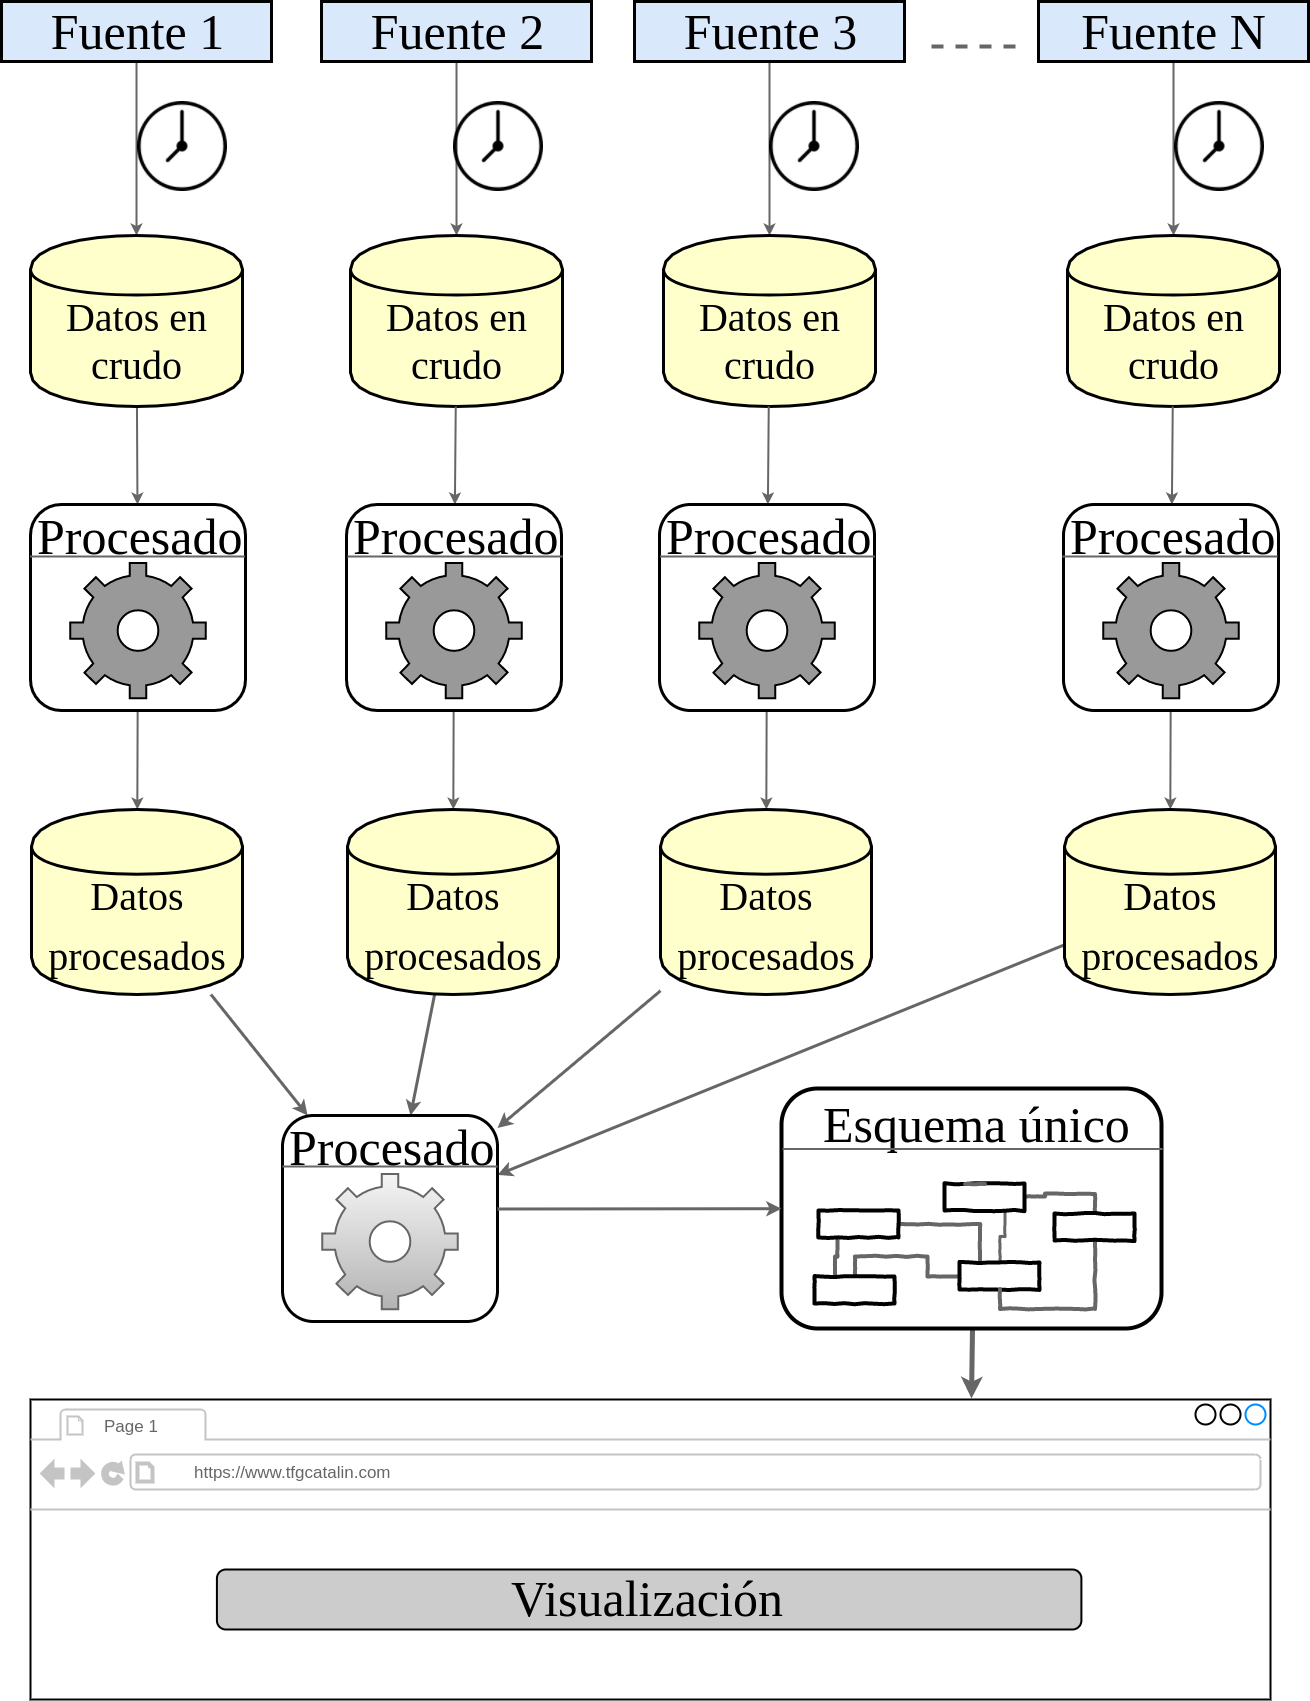
\includegraphics[width=1\textwidth,height=15cm,keepaspectratio]{Imagenes/disenyoconceptual}
    \caption{Diseño conceptual de la solución}
    \label{fig:disenyoconceptual}
\end{figure}




\section{Diseño final} \label{disenyo.final}



En el apartado anterior se ofreció una visión de alto nivel del diseño de la solución, sin hablar de herramientas ni de tecnologías concretas. En este apartado se va a profundizar en el diseño y se va a explicar en detalle la manera en que los datos pasan a través de las diferentes herramientas dentro del sistema, desde la descarga de los datos desde sus fuentes hasta su visualización en pantalla, pasándo por las diferentes etapas de procesado y almacenamiento. 
\par


En el diagrama de la figura \ref{fig:disenyofinal} se puede observar un mapeo casi directo entre los elementos del diseño final y los del diseño conceptual de la figura \ref{fig:disenyoconceptual}. Se puede observar que el diseño final incluye a \textit{Talend Big Data} como responsable tanto de los procesos que descargan y almacenan los \textit{datos en crudo} como de los que posteriormente procesan y almacenan los datos como \textit{datos procesados}. En cuanto al sistema de almacenamiento, que guardará tanto los datos originales como los modificados se utilizará \textit{Apache Hadoop} para los \textit{datos en crudo} y \textit{Apache Hive} dentro de \textit{Apache Hadoop} para los \textit{datos procesados}. Una vez los datos estén transformados y almacenados corréctamente, se usará \textit{Apache Sqoop} para transferirlos a ese esquema único que se persigue como objetivo, y que estará almacenado dentro de una base de datos \textit{MySQL}. Para que este último paso sea posible, debe ser el propio \textit{Talend} quien prepare los datos para ser integrados directamente en el esquema unificado. \textit{JHipster} tendrá una conexión directa a la base de datos \textit{MySQL} y gracias a ello será capaz de leer los datos y mostrarlos en pantalla con su propia interfaz web. 
\begin{figure}[H]
    \centering
    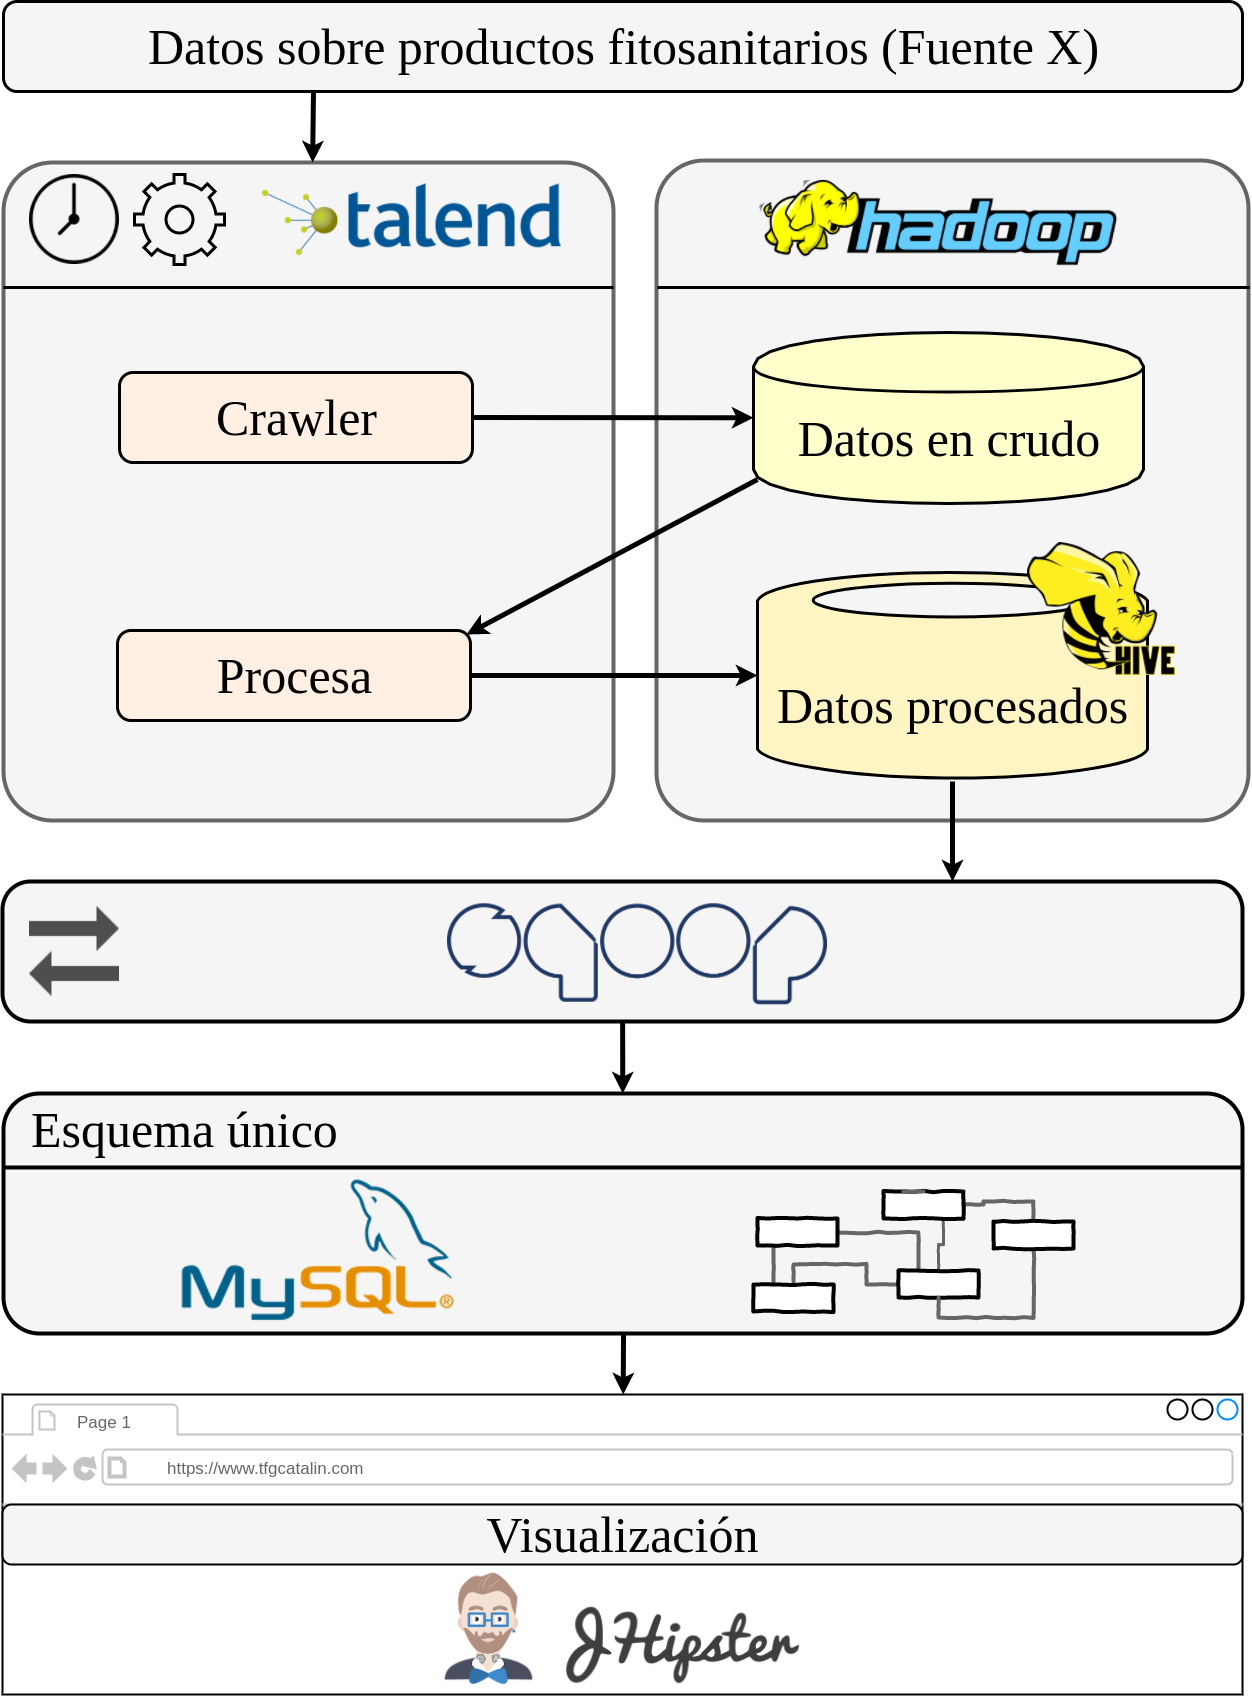
\includegraphics[width=1\textwidth,height=15cm,keepaspectratio]{Imagenes/disenyofinal}
    \caption{Diseño final de la solución - De los datos a su explotación}
    \label{fig:disenyofinal}
\end{figure}

\section{Arquitectura del sistema} \label{disenyo.arquitectura}
\par Este apartado tratará de dar una visión arquitectural del sistema, pasando por diferentes diagramas para representar el proyecto de manera gráfica y completa. Esta sección abarcará los siguientes diagramas: diagrama de despliegue, diagrama de componente y conector, diagrama de clases y paquetes, diagrama de secuencia y diagrama de datos. 

\subsection{Diagrama de despliegue.} \label{disenyo.arquitectura.despliegue}
\par Como se puede observar en la figura \ref{fig:despliegue}, el despliegue de la aplicación consta de un nodo principal, el Servidor. Este almacena tanto la aplicación de \textit{JHipster} como la base de datos \textit{MySQL} y \textit{Apache Sqoop}. La aplicación de \textit{JHipster}, al tratarse de una aplicación \textit{Spring} se representa como un artefacto dentro de un contenedor \textit{Spring}, el \textit{Spring Container}. Además, allí se define el módulo de \textit{schedulling} implementado por el alumno como un artefacto separado del de la aplicación, aunque a nivel práctico realmente su implementación está ubicada dentro del propio módulo de la aplicación. \textit{Apache Hadoop} aparece en el diagrama como una \textit{base de datos} aparte, por varias razones: en primer lugar, \textit{Apache Hadoop} se puede desplegar en un nodo separado del Servidor. En segundo lugar, se pueden crear varias instancias en diferentes nodos del mismo para conseguir almacenar una cantidad mayor de datos, y proporcionar la aplicación de un componente de almacenamiento escalable.
\begin{figure}[H]
    \centering
    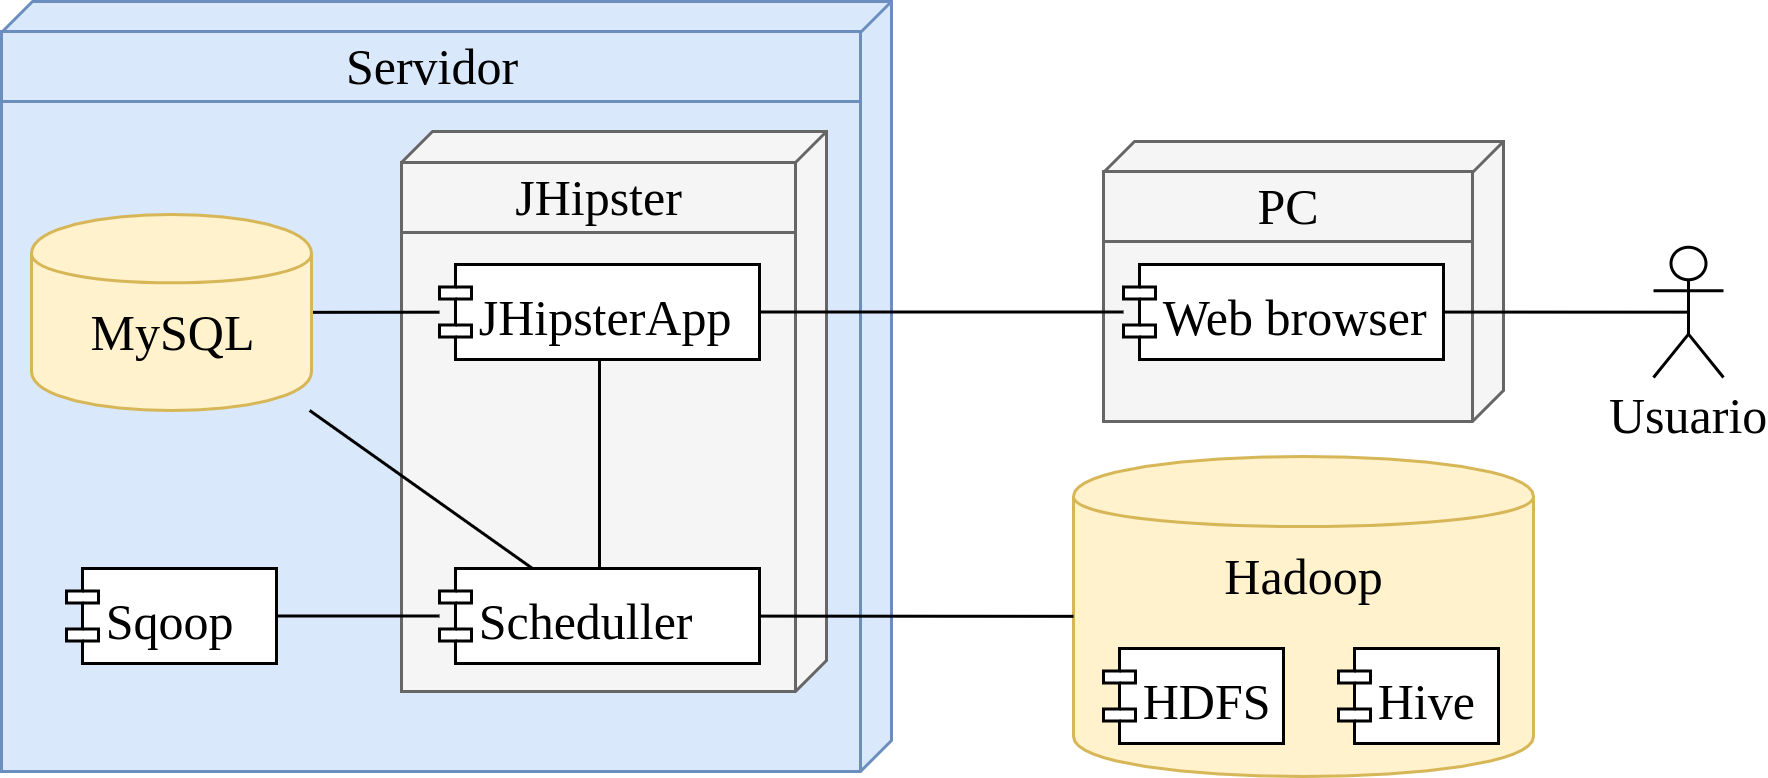
\includegraphics[width=1\textwidth,height=15cm,keepaspectratio]{Imagenes/despliegue}
    \caption{Diagrama de despliegue de la solución}
    \label{fig:despliegue}
\end{figure}

\subsection{Diagrama de componente y conector.} \label{disenyo.arquitectura.cyc}
\par El diagrama de la figura \ref{fig:cyc} muestra la visión arquitectural del sistema a nivel de componentes y conectores. En él se representan todos los elementos del sistema junto con las interfaces que ofrecen y utilizan cada uno de ellos. Se observan todas las conexiones que hay entre los distintos componentes y se puede interpretar como una expansión, o una visión de más bajo nivel del diagrama de despliegue. Se entiende el componente \textit{Talend} como los distintos procesos desarrollados con esta herramienta, más que una conexión con el propio programa ya que en ningún momento se requiere de \textit{Talend} más allá que para la construcción de dichos procesos. 

\begin{figure}[H]
    \centering
    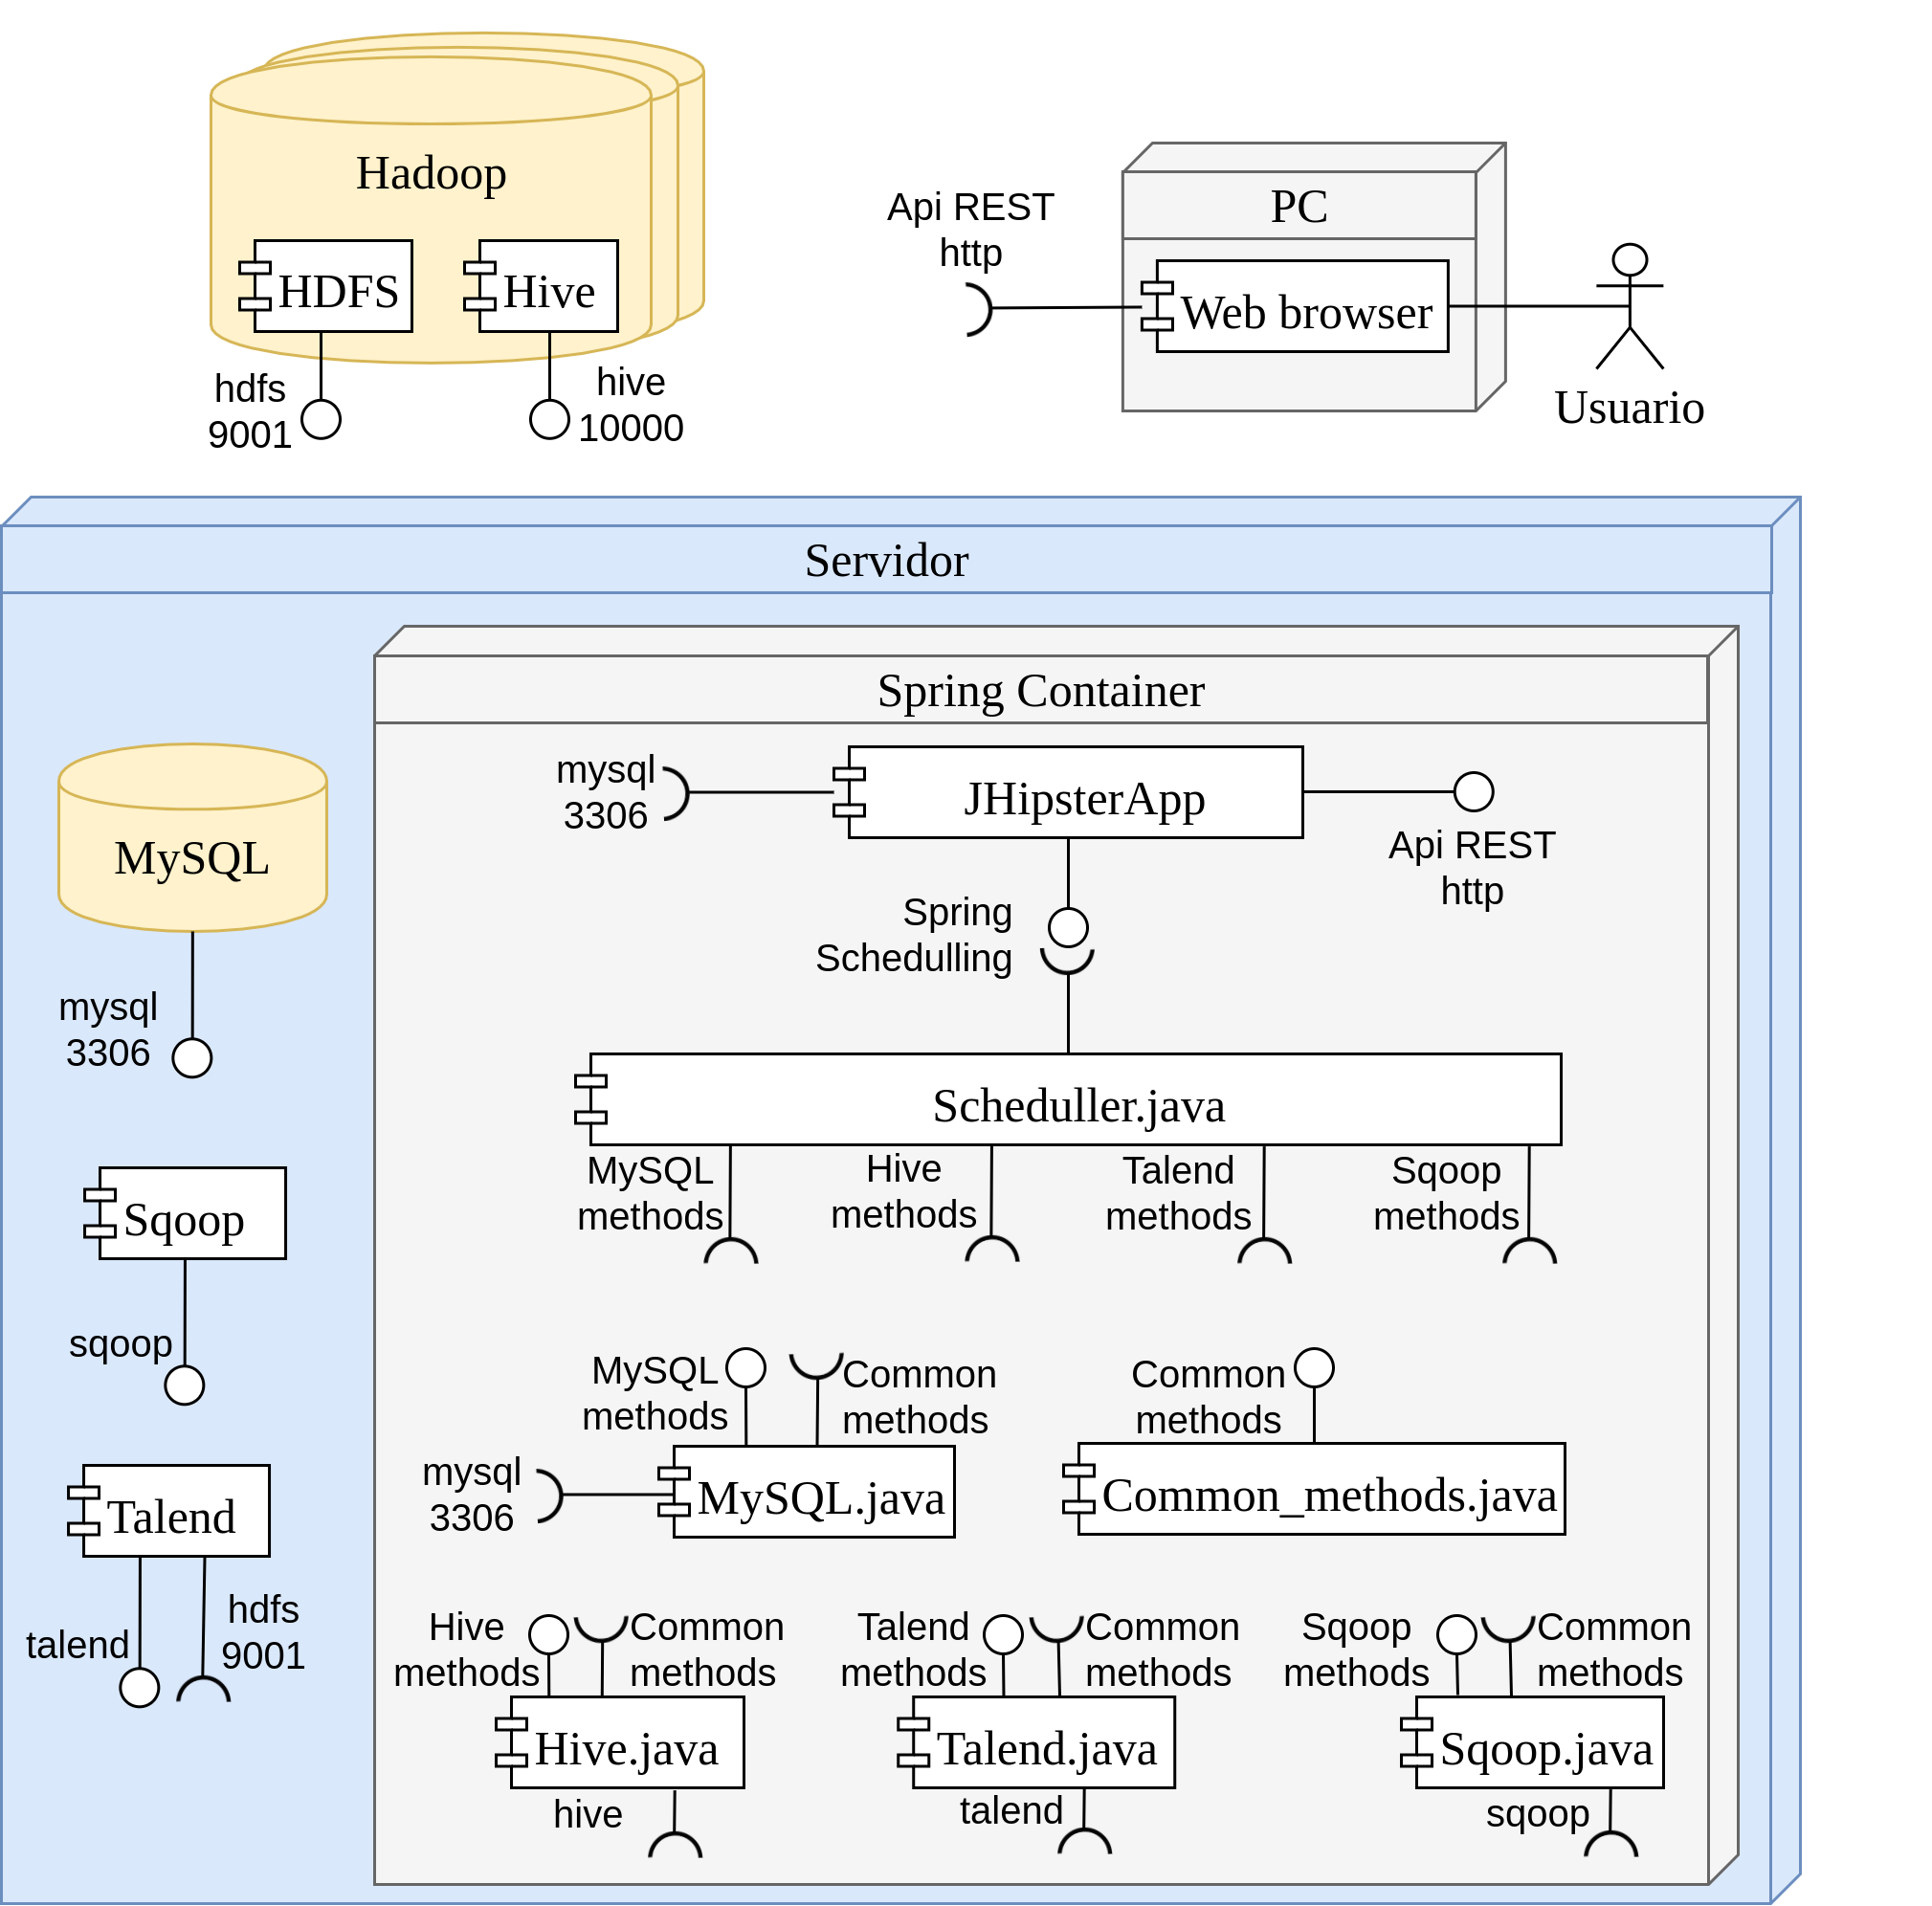
\includegraphics[width=\textwidth,height=\textheight,keepaspectratio]{Imagenes/cyc}
    \caption{Diagrama de componente y conector}
    \label{fig:cyc}
\end{figure}


\subsection{Diagrama de clases y paquetes.} \label{disenyo.arquitectura.clases}
 En el diagrama de clases presente en la figura \ref{fig:diag_clases} se adjunta el modelo de clases y paquetes correspondiente a la infraestructura que se construyó para soportar el comportamiento mencionado en la sección Implementación del prototipo real (Sección  \ref{implementacion.prototipo}). Dicho diagrama no incluye aquellas partes del código que se generan durante la instanciación de la aplicación con \textit{JHipster} sino únicamente las que el alumno ha desarrollado. 


\begin{figure}[H]
    \centering
    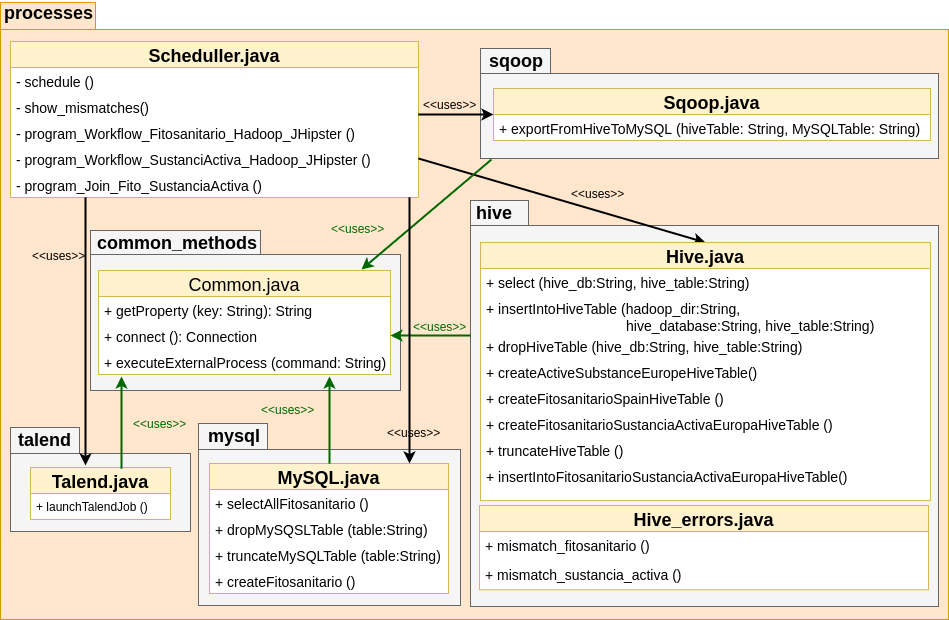
\includegraphics[width=\textwidth,height=\textheight,keepaspectratio]{Imagenes/clases}
    \caption{Diagrama de clases y paquetes para soportar la automatización del \textit{workflow}}
    \label{fig:diag_clases}
\end{figure}

\subsection{Diagrama de secuencia.} \label{disenyo.arquitectura.secuencia}
\par Una vez vista la estructura del diagrama anterior, a continuación se presenta un diagrama de secuencia de ejemplo para ilustrar la interacción de los diferentes componentes y el rol que juegan en el \textit{workflow} desde que los datos se descargan hasta que pasan a visualizarse mediante \textit{JHipster} Para ello se ha hecho uso de un ejemplo \textit{vertical} para los datos de los productos fitosanitarios autorizados de España. Periódicamente, los datos se descargan desde la web del \textit{MAPAMA} \cite{mapama}, son procesados y almacenados en \textit{Apache Hadoop}, se exponen en \textit{Apache Hive}, se transfieren con \textit{Apache Sqoop} a \textit{MySQL} y \textit{JHipster} es capaz de visualizarlos.

\begin{landscape}
\begin{figure}[p!]
    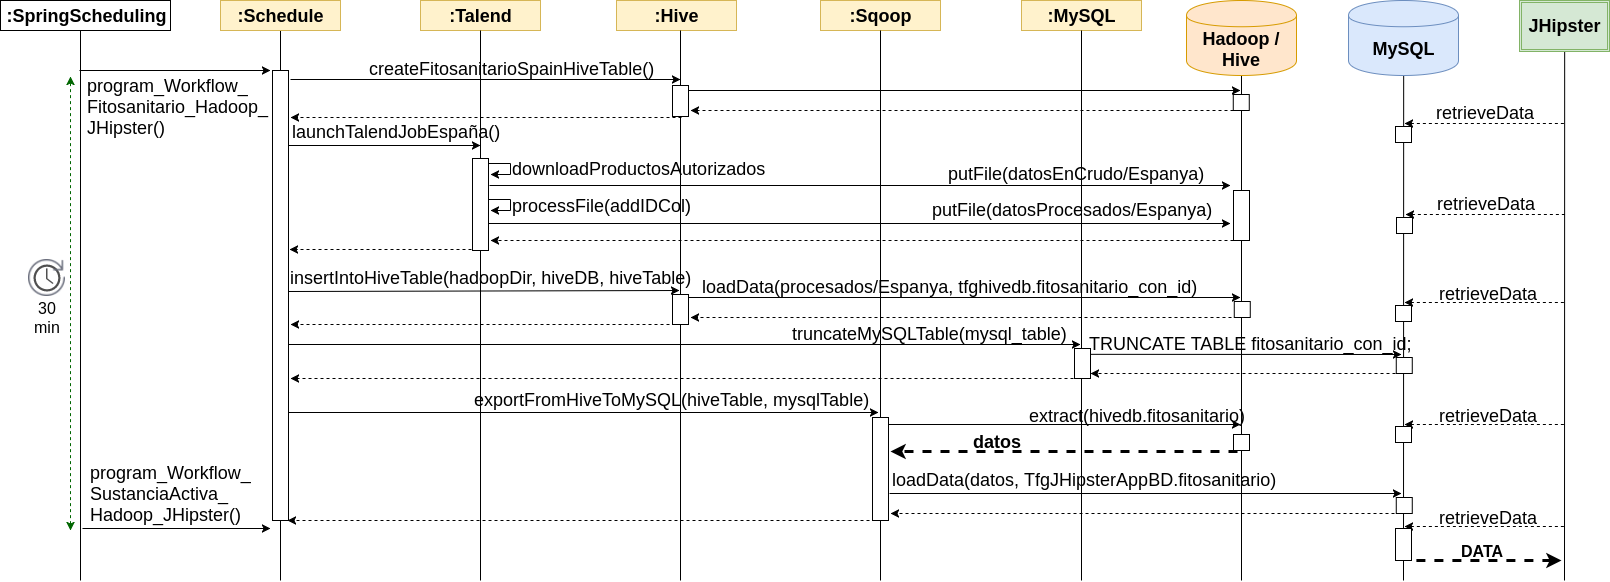
\includegraphics[width=\linewidth]{Imagenes/secuencia}
    \caption{Diagrama de secuencia del \textit{workflow} implementado}
    \label{fig:diag_secuencia_workflow}
\end{figure}
\end{landscape}
\bigskip


\subsection{Diagrama de datos.} \label{disenyo.arquitectura.datos}
\par A continuación se muestra el diagrama de datos tal como están almacenados en \textit{Apache Hive}. A pesar de que también se almacenan datos en la base de datos \textit{MySQL}, la estructura presente allí es relativamente sencilla en comparación con la de \textit{Apache Hive} y por lo tanto se ha decidido presentar en los anexos, en la sección \ref{a.datos.modelo}. 
\par 
Como se puede observar, en la figura \ref{fig:datosApache Hive} aparecen, mediante una estructura de diagrama entidad-relación las entidades que han sido creadas en \textit{Apache Hive}. Por una parte tenemos las entidades \textit{fitosanitario\_con\_id} y \textit{sustancia\_activa\_europa}, que son las entidades principales de la solución. La primera se crea a partir de los datos obtenidos de la primera fuente integrada en el proyecto, proveniente del listado de productos fitosanitarios autorizados en España disponibles en la página web del \textit{MAPAMA} \cite{mapama}. La segunda son los datos de las sustancias activas provenientes de la base de datos abierta sobre pesticidas a nivel europeo. El resto de entidades presentes en el modelo son el resultado de diferentes operaciones sobre estas dos tablas. A continuación se explica cómo se han conseguido dichas entidades y qué representan. 
\begin{enumerate}
\item En primer lugar, la relación marcada con un \textit{1} en el diagrama representa una cierta similitud en el campo \textit{formulado} de la primera tabla y el campo \textit{name} de segunda: El \textit{formulado} incluye el \textit{name} de la segunda tabla. No obstante, los datos no son perfectos: por una parte está el problema del idioma; muchos de los fitosanitarios aparecen en español mientras que las sustancias activas están en inglés, por lo que un mapeo directo no daría el 100\% de los \textit{matches}. Otro problema es el de los \textit{campos múltiples}, esto es, en la primera tabla, algunos registros del campo \textit{formulado} incluyen no solo uno, sino varios nombres de sustancias activas. Por lo tanto, haría falta una búsqueda para poder hacer el matching con todas las sustancias activas encontradas.
\item La relación marcada con un \textit{2} representa la tabla \textit{fito\_active\_substance}, que es el resultado de hacer un mapeo casi directo de la relación mencionada en el punto anterior: Primero, del campo \textit{formulado} nos quedamos únicamente con el nombre de la sustancia activa. Después se hace una operación de \textit{JOIN} para conseguir el \textit{real\_id} (id real de la sustancia activa) de la segunda tabla.
\item Las relaciones marcadas con un \textit{3} y un \textit{4} surgen de la necesidad de registrar los errores; las tablas \textit{mismatch\_fitosanitario\_fito\_sustancia} y \textit{mismatch\_sustancia\_fito\_sustancia} recogen aquellos fitosanitarios de la primera tabla que no aparecen en la tabla \textit{integrada} (\textit{fito\_active\_substance}) y aquellas sustancias activas de la segunda tabla que tampoco aparecen, respectívamente.
\end{enumerate}

\begin{landscape}
\begin{figure}[p!]
    \centering
    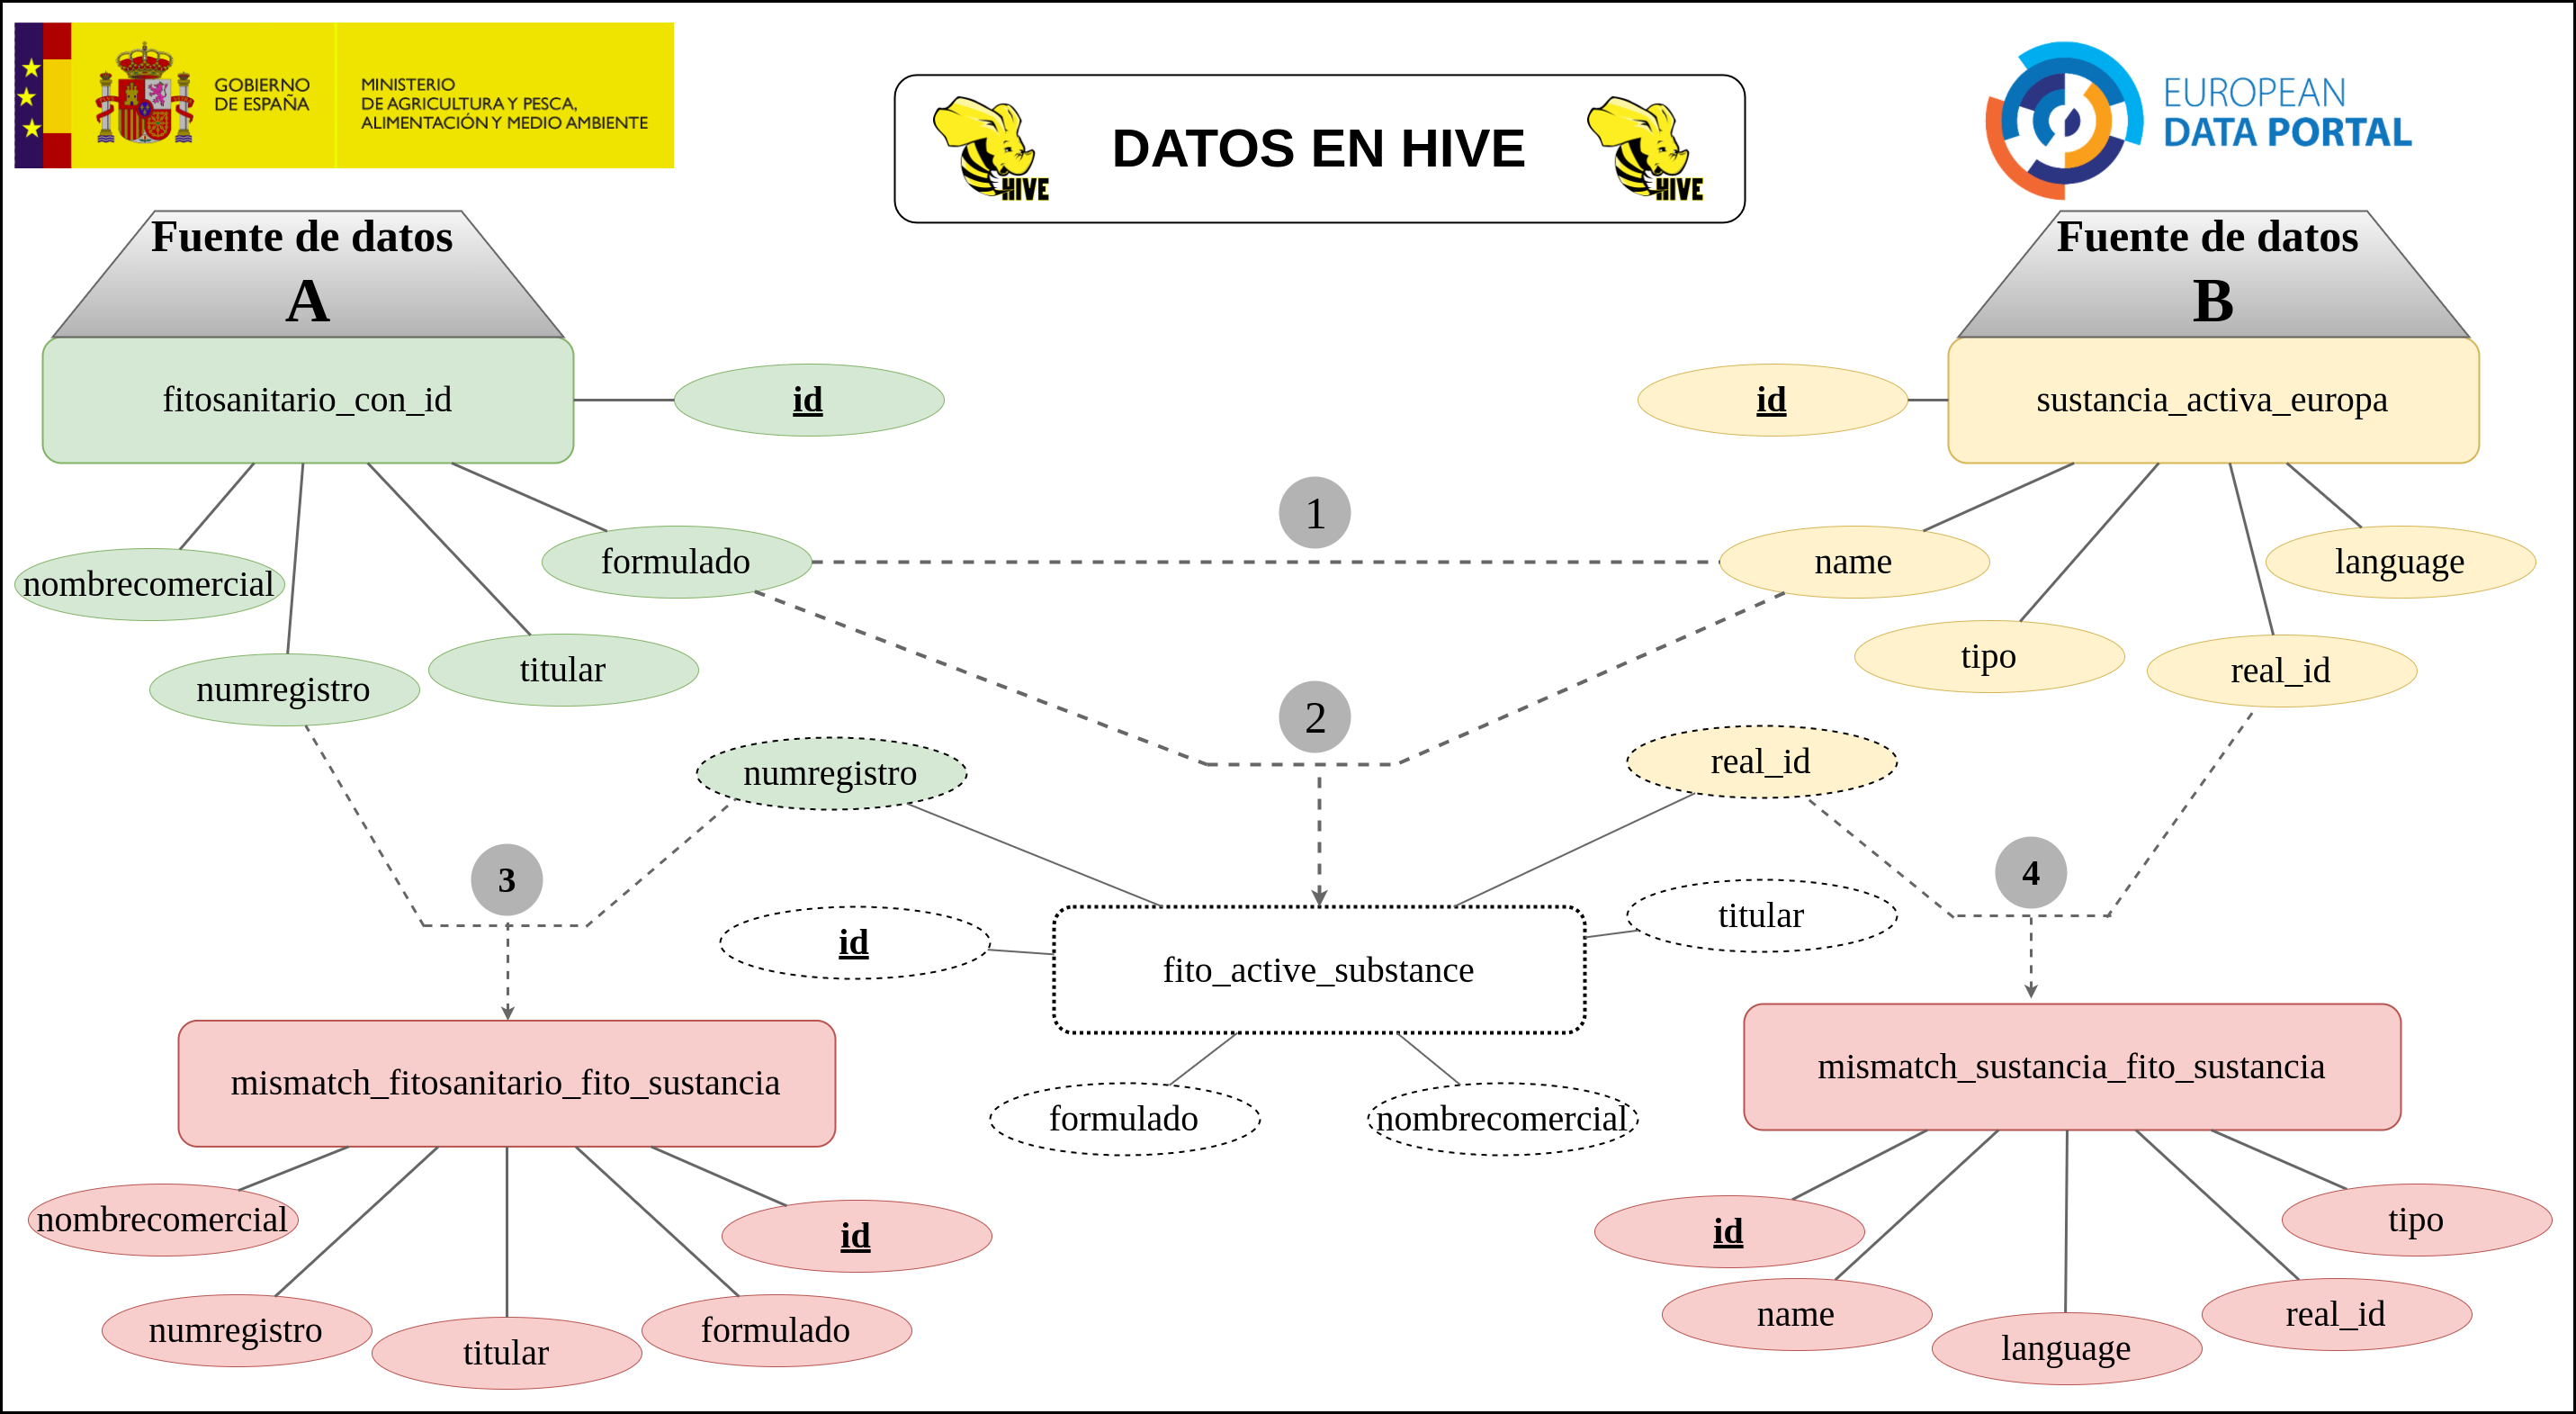
\includegraphics[width=\linewidth]{Imagenes/datoshive}
    \caption{Esquema de datos importados en \textit{Apache Hive}}
    \label{fig:datosApache Hive}
\end{figure}
\end{landscape}





\section{Estrategia de integración y expansión}
\label{disenyo.estrategia}

Una vez visto el diseño del sistema, en esta sección se hablará de la estrategia de integración y expansión que gobernará los futuros desarrollos a partir de la infraestructura montada en la realización de este proyecto. 

Como se observará en el desarrollo del prototipo real de la sección \ref{implementacion.prototipo}, realmente gracias a la infraestructura conseguida y a la arquitectura que se ha montado, realizar nuevas funcionalidades y expandir el proyecto no debería suponer un reto y debería ser bastante asequible. En este apartado caben destacar varias líneas posibles de expansión en el proyecto: 

\paragraph*{Aumento de la capacidad de almacenamiento.} Este apartado es bastante trivial, puesto que gracias a \textit{Apache Hadoop}, esto se puede conseguir fácilmente. Tal como se ha comentado, \textit{Apache Hadoop} tiene el potencial de crecimiento mediante nodos adicionales, desplegados en la misma o en diferentes máquinas, con capacidad de almacenamiento extra. Así pues, para que el sistema escalase en cuanto a capacidad de almacenamiento, lo único que se tendría que hacer es desplegar más nodos de \textit{Apache Hadoop} para tener la información repartida en más espacio de almacenamiento. 

\paragraph*{Integración de datos nuevos.} Para integrar nuevos datos en el sistema de nuevas fuentes, la estrategia a seguir debería ser la que se observa en el diagrama de la figura \ref{fig:expansion}.

\begin{figure}[!h]
    \centering
    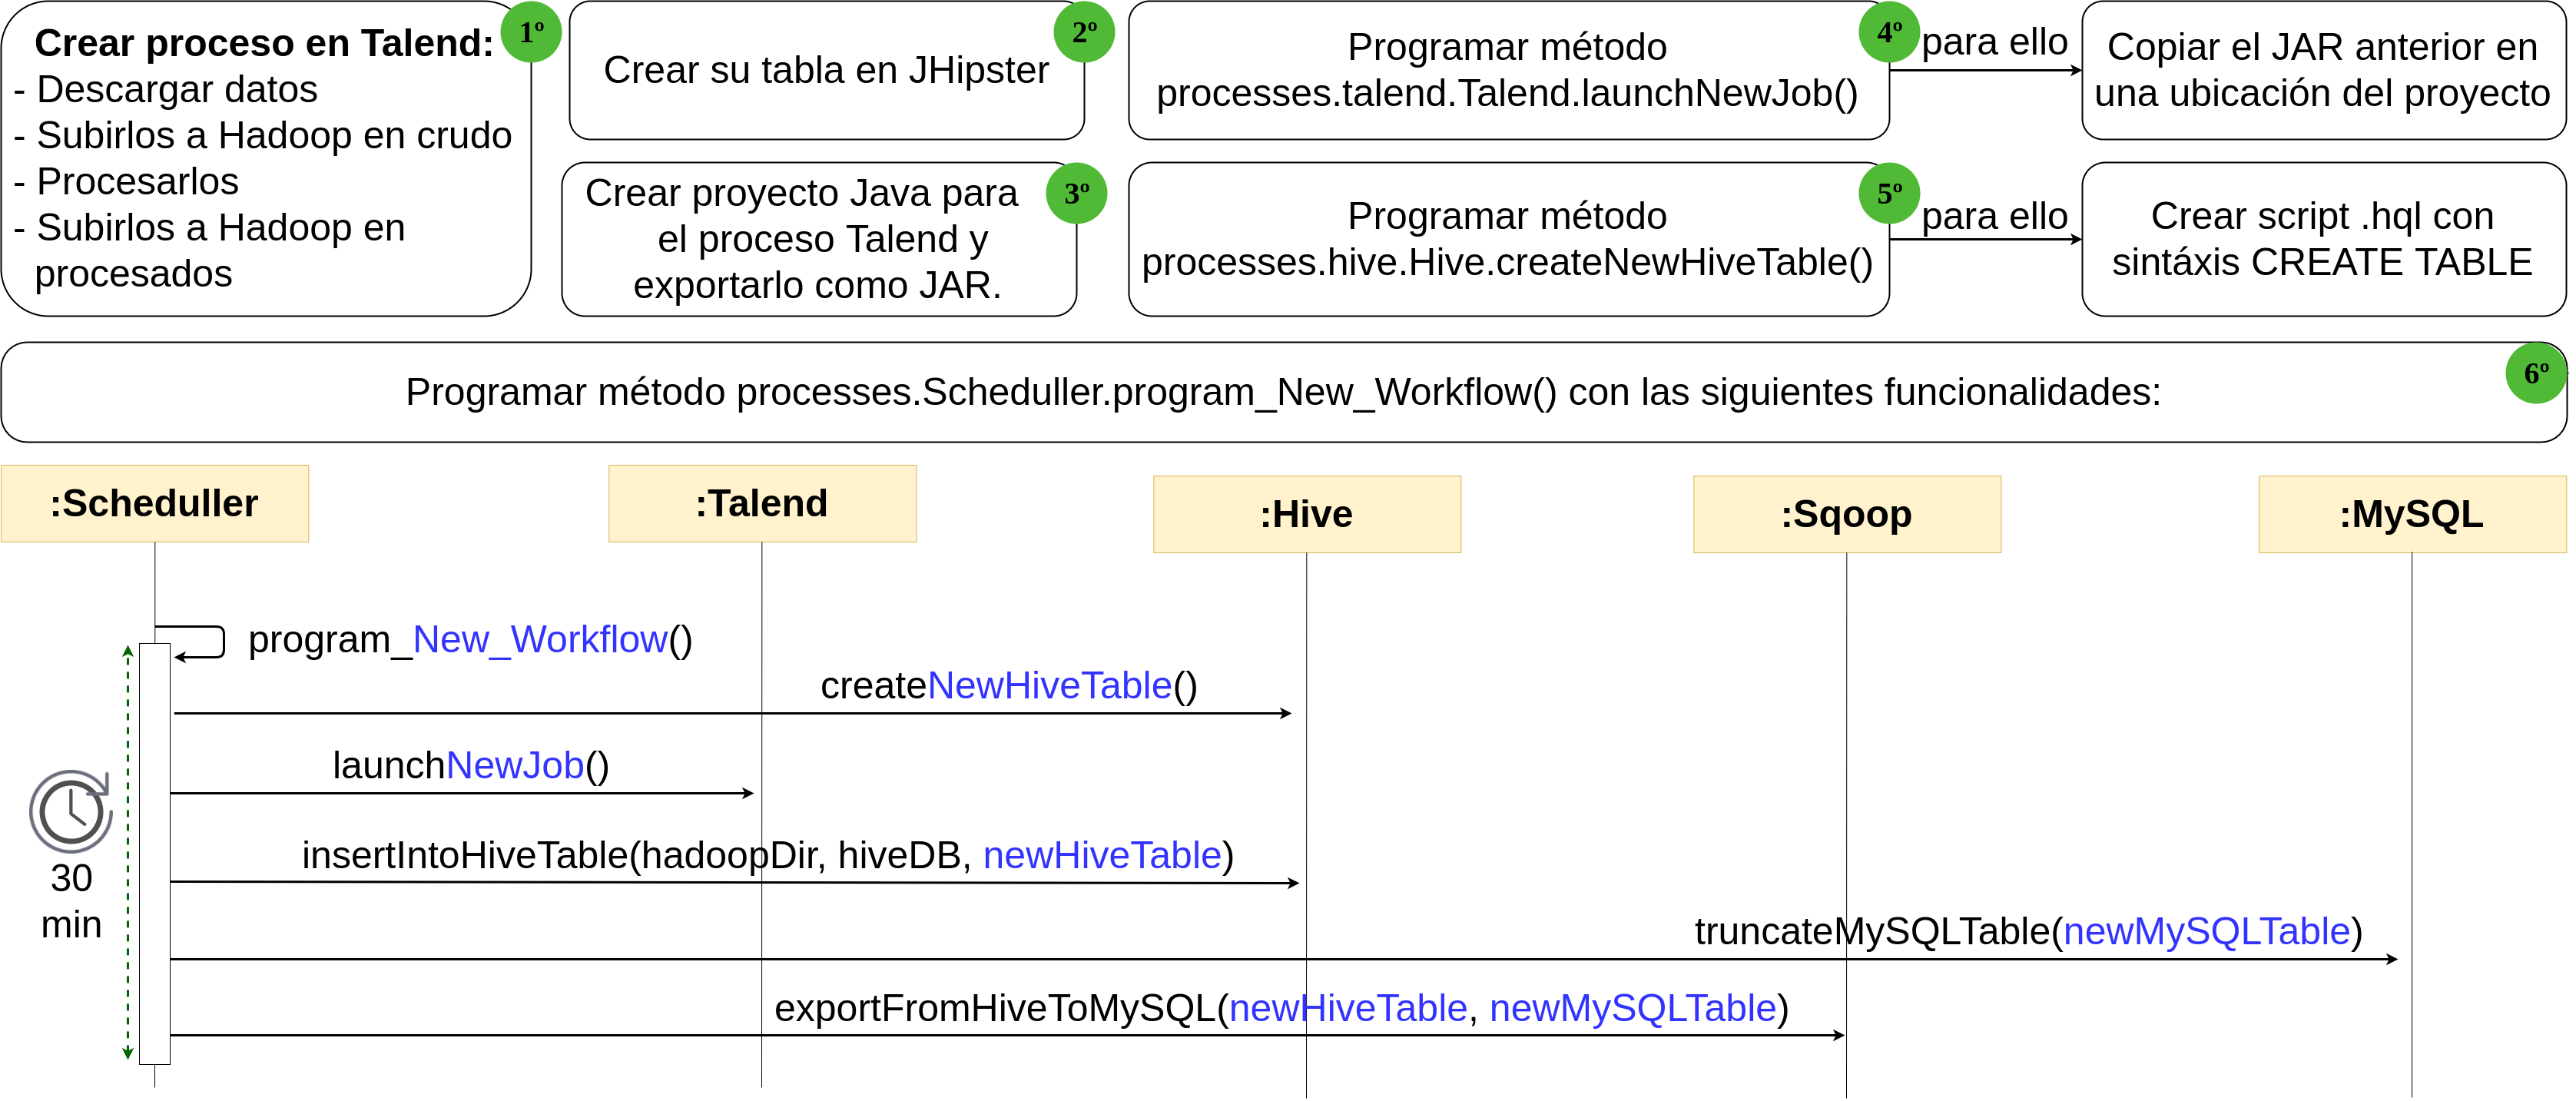
\includegraphics[width=\textwidth,height=\textheight,keepaspectratio]{Imagenes/expansion}
    \caption{Estrategia recomendada para la integración de datos nuevos}
    \label{fig:expansion}
\end{figure}
\textbf{Funcionalidades extra.} Aunque realmente este proyecto se ha desarrollado pensando en una expansión futura únicamente en cuanto a la integración de nuevos datos y la escalabilidad de almacenamiento, gracias a la estructura de la aplicación de \textit{JHipster} es posible dotar al sistema de tantas funcionalidades extra como se desee. 

\section{Restricciones al diseño} \label{disenyo.restricciones}
La gestión y desarrollo del proyecto, en todas sus fases se ha visto restringida por diferentes pautas y recomendaciones provenientes de terceras partes. Este apartado pretende aclarar algunas de estas cuestiones para reflejar aquellas decisiones que han condicionado, para bien o para mal, el desenvolvimiento del alumno. 
\par Desde el inicio del proyecto el director impuso algunas de las herramientas a utilizar, así como el diseño a priori de la solución. \textit{Apache Hadoop}, \textit{Apache Hive} y \textit{JHipster} fueron el \textit{core} tecnológico que el director estableció para la realización del proyecto. Como primer diseño, además, el director expuso un modelo en el que los datos tanto procesados como sin procesar serían almacenados en \textit{Apache Hadoop}, consumidos desde \textit{Apache Hive} e importados directamente a \textit{JHipster}, sustituyendo la base de datos de \textit{JHipster} por \textit{Apache Hive}. Tras observar que este modelo no cumplía con los requisitos del proyecto, se optó por la otra variante, mediante \textit{Apache Sqoop}, tal como se ha mencionado anteriormente. 
\par Otra de las herramientas recomendadas por el director del proyecto fue \textit{Pentaho Kettle} y, como se puede observar en la sección \ref{implementacion.problemas}, fue una de las piezas que más problemas acabó dando. Ante esta situación, el director recomendó \textit{Talend}, que resultó ser un mejor componente y que satisfacía con los requisitos de la fase de análisis.
\par Otro aspecto que se debe tener en cuenta es que el proyecto se trata de un \textit{TFG} y no de una solución comercial. Por ello, hay unas normas o pautas  establecidas que delimitan y guían en el desarrollo del mismo: la limitación de las horas de dedicación recomendadas, que se corresponden a los 12 créditos ECTS, la inclusión de una memoria suficientemente extensa para recopilar todos los aspectos del desarrollo del proyecto e incluso la limitación económica implícita, esto es, no existe una remuneración monetaria para el alumno tras el desarrollo del proyecto. 





